\documentclass[lang=cn,10pt]{elegantbook}

\title{智弈锋穹--AI驱动的攻防自治演训靶场}
\subtitle{项目文档}

\author{网安院十个人}
\bioinfo{指导老师}{张立强、何艺、严飞}
\institute{武汉大学 国家网络安全学院}
\date{2025年8月14日}

% \extrainfo{不要以为抹消过去,重新来过,即可发生什么改变。—— 比企谷八幡}

\setcounter{tocdepth}{3}

% \logo{cyber-4084719_1280.jpg}
\cover{cyber-4084719_1280.jpg}


% 本文档命令
\usepackage{array}
\newcommand{\ccr}[1]{\makecell{{\color{#1}\rule{1cm}{1cm}}}}

% 修改标题页的橙色带
\definecolor{customcolor}{RGB}{7,8,8}
\colorlet{coverlinecolor}{customcolor}

\begin{document}

\maketitle
\frontmatter

\tableofcontents

\mainmatter


\chapter{项目背景和概述}
\begin{introduction}
    \item 赛题背景
    \item 基本知识背景
\end{introduction}

\section{赛题背景}

党的十八大以来,以习近平同志为核心的党中央高度重视网络安全工作,特别在目前日趋复杂
的背景下,深刻认识和有力防范网络安全风险,切实维护网络空间安全,已成为事关全局的重大课
题。

随着《网络安全法》和《国家网络空间安全战略》的深入推进,
实战化网络攻防能力的建设成为网络安全体系中的关键任务之一,
尤其在“十五五”规划对关键信息基础设施安全防护提出更高要求的背景下,
传统的网络安全演练方式已难以满足动态演训和智能对抗的发展趋势,
目前在实际操作中面临三方面的主要瓶颈:

一是传统靶场场景构建模式过于静态,往往采用人工预设的方式搭建演练环境,
更新周期长、调整代价高,导致其难以及时引入现实世界中快速变化的业务架构、
操作流程以及技术组件,也无法涵盖近年来不断涌现的新型攻击方式与复杂威胁模型,
例如APT、供应链渗透、0day漏洞利用等,
这种脱节使得演练内容始终滞后于现实威胁的发展态势,
无法为参与者提供贴近实战的演练体验,也难以检验系统和人员在面对未知攻击时的应对能力,
从而削弱了靶场演练在实战能力培养中的实际价值。

二是攻击路径往往依赖人工预设,主要根据经验规则构建固定的攻击链条,
缺乏动态生成机制与策略调整能力,导致攻击行为表现出明显的模式化特征,
不仅在路径选择上缺乏多样性,也难以模拟出真实渗透过程中攻击者面对防护机制时的适应性调整与策略转移,
无法体现现代网络攻防中攻击面广泛、路径不确定、阶段交错的复杂局面,
这种设计上的单一性和僵化性直接削弱了演练的覆盖广度与挑战强度,
最终造成演练内容与现实渗透行为之间出现严重脱节。

三是评估机制普遍依赖人工回顾,
主要通过事后分析操作日志、观察系统响应或专家打分等方式进行效果判断,
不仅耗时耗力,而且评判结果高度依赖评估人员的主观判断,
缺乏统一的标准与可复用的指标体系,难以保障结果的一致性与公正性,
也制约了后续能力提升、策略优化与人才选拔的科学性与有效性。

这些问题在一定程度上制约了演练体系的有效性和可持续发展,
因此亟需以网络攻防动态推演为核心突破口,
引入AI Agent、数据分析与自动化决策等新技术,
实现演练环境的动态演化、攻击过程的智能模拟、
防御策略的自适应优化以及评估体系的全面量化,
从根本上提升攻防演练的实效性与科学性,推动网络安全实战能力建设迈上新台阶。

\section{基本知识背景}

\subsection{KVM虚拟机}

KVM是一种内建于Linux内核的虚拟化技术,
它将Linux操作系统转变为一个完整的Type-1虚拟化管理程序。
KVM依赖硬件虚拟化扩展(如Intel VT或AMD-V)来为每个虚拟机提供
独立的虚拟CPU和内存资源,并通过QEMU作为后端模拟设备和系统行为,
从而运行不同操作系统的虚拟实例。每台虚拟机以普通进程的形式运行在宿主机上,
由内核模块kvm.ko管理其特权指令的捕获与转发。KVM虚拟机具备高性能和低开销的特点,
支持资源动态分配、快照保存、虚拟网络构建等功能,适合用于构建多租户的复杂网络环境。
通过Libvirt工具集与Virt-Manager图形界面,
用户可以以更直观和统一的方式对虚拟机生命周期进行管理,
显著简化了大规模虚拟基础设施的运维难度。

\subsection{Docker容器}

Docker是一种轻量级虚拟化技术,
它通过操作系统级别的内核功能如命名空间和控制组来实现对进程的隔离与资源限制。
容器运行在共享内核的宿主机上,但对每个容器而言,它拥有独立的文件系统、网络堆栈
与进程空间。Docker镜像作为容器的模板,以分层文件系统构建,支持快速部署与复用,
显著提升了环境一致性和服务交付效率。
相较于虚拟机,容器启动速度更快、占用资源更少,更适合部署短周期、可弹性伸缩的服务。
在靶场环境中,Docker通常用于承载Web服务、数据库、日志分析平台等高频变化的组件,
通过Docker Compose工具可实现多容器服务的集中编排,提升整体自动化部署水平。

\subsection{靶场建构及其自动化}

靶场系统通过KVM虚拟化技术构建多个相互隔离但逻辑互通的虚拟网络,
旨在还原现实企业网络的典型结构与安全边界。系统整体以宿主机为核心,
借助网络编排规则和NAT功能对不同区域的流量进行统一调度和安全控制,
形成了完整的攻防演练环境。

外部攻击流量首先从互联网进入宿主机的物理网卡(如eth0),
宿主机通过配置DNAT规则将特定端口的流量重定向至虚拟网络net-ext中的跳板机或VPN服务器。
net-ext充当外部网络的模拟区域,其内主机可借助宿主机NAT访问真实互联网,
具备基础的对外通信能力。

处于安全缓冲区位置的net-dmz网络承担DMZ区域职能,
部署有Web服务器与邮件服务器等对外服务资产。
这些主机通过宿主机的网络编排规则接受来自net-ext的受控流量,
同时具备访问内部网络数据库的权限。DMZ区域的配置兼顾开放性与安全性,
是攻击链中的核心跳板节点之一。

net-int网络模拟企业内部办公网,
主要部署PC终端、数据库服务器及业务支撑服务。该区域强调防护强度,仅允许向外发送请求,
拒绝绝大多数来自外部与DMZ区域的主动连接,内部主机仅接受来自DMZ内特定主机的数据库访问请求。
net-int作为攻击链的最终目标区域,其安全策略最为严格。

net-mgmt为管理专用网络,部署KVM管理节点、日志分析平台、安全监控系统等支撑资产。
该网络通过带外方式管理其他所有网络中的主机与容器,不参与业务流量传输,
与其它区域完全逻辑隔离。net-mgmt的存在确保了运维操作的独立性与安全性,
是演练过程中分析与干预的关键通道。

上述各网络间通过宿主机实现隔离与流量控制,同时具备有限的、策略可控的访问路径。
这种多层级、区分角色的网络架构能够精细复现企业级生产网络的安全边界与访问关系,
为红队攻击链设计、蓝队监控部署以及后期行为分析提供可信、可控、可观测的环境支持。


\subsection{AI Agent}

AI Agent是一种具备感知、决策与执行能力的自主体,
用于模拟人类在特定任务下的操作行为。
在攻防演练中,Agent通过持续感知环境变化、分析目标系统特征、
结合既有知识进行推理并最终发起攻击或防御行为,体现出智能化对抗的动态性和自适应性。

一个典型的Agent包括感知模块、知识表示模块、策略生成模块和行为执行模块,
其运行过程涉及对目标资产的信息采集、漏洞推理、攻击路径生成和自动化利用。
随着大模型技术的发展,Agent逐渐具备了更强的自然语言理解能力与代码生成能力,
能够从文档、漏洞数据库中抽取并构建攻击利用逻辑。

在本项目中,我们使用了Gemini CLI构建攻防Agent,借助其集成的上下文感知机制、
多模态输入解析能力和代码生成能力,完成对渗透链条的智能模拟与自动攻击脚本的生成,
探索了基于大模型驱动的Agent在靶场环境中的实战应用潜力。


\chapter{项目设计思路与方案}
\begin{introduction}
  \item 项目目标设计思路
  \item 前端设计方案
  \item 靶场基础设施设计方案
  \item 攻击模块设计方案
  \item 防御模块设计方案
  \item 评价模块设计方案
  \item 模块协同设计
\end{introduction}
\section{项目目标设计思路}
攻击防御评价系统的目标设定,
源于网络安全演练领域的核心痛点:传统演练多依赖人工搭建环境、手动记录过程,
存在场景单一、评估主观、效率低下等问题。
基于此,系统目标聚焦于构建 “全流程数字化演练平台”,
通过拓扑结构展示、AI Agent驱动的攻击演练、自动化评估三大核心功能,
实现从环境搭建到结果分析的闭环管理。​

\begin{theorem}
    前后端数据实时交互,杜绝因信息延迟影响演练效果。
\end{theorem}

从功能边界来看,前端与后端的拆分遵循展示与控制分离的设计原则。
前端主要负责构建可视化的交互界面,包括资源监控平台和模拟终端,
便于用户直观了解网络运行状态和攻击演进过程,
增强了用户的操作体验和对演练环境的理解程度,
而后端则不仅承担着靶场底层拓扑结构的可调整参数的搭建与管理,
确保整个系统运行的稳定性与评估指标的客观性,
同时还集成了AI Agent自主攻击模块、防御控制模块
以及完整的演训日志记录系统,
使得整个平台具备自动化、智能化的攻防能力和可审计的追踪能力,
这种架构设计不仅有效满足了用户在操作便捷性方面的需求,
也充分保障了平台在功能性、扩展性与安全性方面的可靠性,
最终形成了一个高效、智能、可信的网络安全实战演练平台,
为防护能力的验证与提升提供了可量化、可复现、可定制的技术依据。

\begin{definition}
    明确系统旨在解决传统演练痛点:

    方案布局上,通过 “可调参数的基础设施 + AI赋能的行为演训” 破除
    传统靶场痛点难题;

    设计架构上,通过 “前端展示 + 后端控制” 架构实现
    全流程数字化可视化闭环管理。
\end{definition}

\section{前端部分设计方案}
前端设计的核心矛盾在于 “动态场景多样性” 与 “前端展示架构稳定性” 的平衡。
为解决这一矛盾,方案采用 “大模型生成 + 预设框架约束” 的混合模式,
既发挥大模型在动态内容生成上的优势,又通过框架控制不确定性。​


在内容生成层面,选择大模型的核心原因是应对复杂网络场景的多样性需求。
网络拓扑、攻击路径等展示内容需根据用户输入的业务场景动态调整,
大模型可基于预设规则生成符合逻辑的可视化元素,大幅降低手动绘制的成本。
但大模型生成存在随机性,因此引入预设框架作为约束 —— 基于 Vue 或 React 构建组件库,
包含拓扑图组件、攻击流程时间轴、评估结果仪表盘等标准化模块,
确保生成内容在布局、交互逻辑上的一致性。​

交互设计上,采用 “打勾选项 + 输入框” 的组合模式提升灵活性。打勾选项覆盖 80\% 的常用功能,如 “显示漏洞节点”“高亮攻击路径” 等,降低用户操作门槛;输入框则支持自定义需求,如 “添加自定义业务系统图标”“修改拓扑连线样式” 等,满足个性化场景。同时,界面美观性通过 “分层视觉设计” 实现:底层为网络拓扑基础图层,中层为攻击 / 防御动态效果层,顶层为操作交互层,配合蓝白主色调(体现专业性)与红黄绿警示色(区分攻击、正常、防御状态),确保运维与安全人员能快速捕捉关键信息。

\begin{definition}
    前端通过 “大模型 + 预设框架” 平衡动态性与稳定性,交互设计兼顾易用性与个性化,
    视觉分层提升信息获取效率。
\end{definition}

\section{靶场基础设施设计方案}


后端设计以 “高可用、可扩展、国产化兼容” 为核心原则,通过容器化架构与国产化技术栈,支撑前端场景的动态运行与核心功能的实现。​

容器编排与部署层面,选择 Kubernetes 作为核心引擎,因其具备强大的容器调度、扩缩容能力,可根据演练规模自动调整资源分配 —— 例如,当攻击演练涉及 100 个节点时,Kubernetes 能快速拉起对应数量的容器实例,避免资源浪费。底层操作系统选用 OpenEuler,不仅因其开源稳定性,更重要的是适配国产化硬件(如鲲鹏处理器),满足关键领域对 “自主可控” 的要求。在兼容性验证上,通过搭建鲲鹏服务器测试环境,对容器启动速度、网络吞吐量等指标进行压力测试,确保在国产化平台上的性能损耗低于 10\%。​

网络拓扑与漏洞环境构建是后端的基础能力。采用 SDN(软件定义网络)技术创建虚拟网络拓扑,支持自定义子网划分、路由规则配置,模拟企业内网、DMZ 区等复杂网络环境。漏洞版本服务部署通过 “镜像仓库 + 版本管理” 实现:将包含不同漏洞的服务(如存在 Log4j 漏洞的 Tomcat、Heartbleed 漏洞的 OpenSSL)封装为标准化容器镜像,存入私有仓库,用户可通过前端选择漏洞类型,后端自动拉取对应镜像并部署,确保每次演练的漏洞环境一致性。​

攻击路径自动化分析是后端核心逻辑,采用 “图论算法 + 漏洞评分体系” 实现。将网络节点视为图的顶点,节点间的连接视为边,通过深度优先搜索(DFS)遍历潜在攻击路径;同时,结合 CVSS 漏洞评分与 Exploit 可用性(如是否存在公开 PoC),对每条路径的 “攻击成功率” 进行量化计算,为自动化评估提供数据支撑。

\begin{definition}
    aaa
\end{definition}

\section{攻击模块设计方案}

\subsection{关键场景攻击链构建}

攻击模块设计以模拟真实网络环境中的典型高级持续性威胁为目标,
打勾选取基础场景,通过构建完整的攻击链路,
展示从初始渗透到数据窃取的全过程。在渗透阶段,
AI Agent将尝试执行社会工程攻击或已知漏洞利用以获取初始访问权限;
在横向移动阶段,攻击体主动识别内网结构,渗透并控制更多节点,
扩大攻击面;在数据窃取阶段,模拟攻击者对已入侵主机进行文件扫描与关键数据提取,
目标文件人工预设于用户目录下,以增强演练的真实性与针对性。
整个过程由攻击AI Agent主导执行,路径选择具备自主决策能力,
可根据目标系统环境自动调整策略,反映出复杂攻击链在真实场景中的演化过程。

\subsection{人工辅助漏洞利用与EXP构建流程}

除自动化攻击路径外,系统也支持人工参与的漏洞利用流程,
用于检验攻击分析能力与EXP生成能力。在内核层面,
演练人员可选择已知存在或根据实际生产环境构建的高危漏洞的虚拟机镜像。

对于nday漏洞演练:
通过调试与运行验证EXP的有效性;在Web服务层面,结合xray和nuclei等漏洞扫描工具,
对目标站点进行扫描与信息收集,识别存在的安全隐患,
并在社区或数据库中查找已公开的PoC,修改参数以适配当前演练环境,
从而实现漏洞的成功利用。整个过程强调人工分析能力与漏洞利用链构建能力的锻炼,
辅助AI Agent形成更完善的攻击库资源。

对于0day漏洞以及APT攻击演练:

\subsection{攻击Agent的自动化执行机制}
我们使用开源Agent客户端框架Gemini Cli作为我们的AI Agent基本架构,
该框架支持多种主流操作系统(如 Windows、Linux、MacOS等),也可适配OpenEuler等国产开源系统。
可配置工作目录自主设置RAG,
并能操作终端执行命令,并自反馈的给出相应回答和调整

为了实现攻击行为的自主执行,攻击Agent具备版本识别、漏洞关联与自动配置功能。
在目标识别阶段,Agent基于资产信息与系统指纹确定目标组件与版本号,
在项目构建的Agent RAG知识检索系统中查找与之对应的已知漏洞信息,并获取匹配的PoC样本;
在利用准备阶段,Agent自动对PoC进行重构与配置,
主要完成攻击目标的地址替换、参数填充与脚本适配;最终执行攻击操作,
并使用Agent log监控其效果反馈,包括系统响应、异常状态与返回值,判断攻击是否成功,
并在必要时根据失败原因调整路径或切换攻击手段,实现攻击链的持续推进与策略自适应。

\subsection{攻击行为自动化评估与结果统计}

为支持攻击模块的自动化评估机制,系统设计了基于日志驱动的攻击效果量化方案,
攻击Agent在每次执行攻击任务时将自动记录完整的行为日志,
包括攻击起始时间、攻击方法、所用PoC编号、尝试次数、目标响应状态与最终效果,
系统对这些数据进行自动归类与统计,生成攻击尝试与成功次数的对比结果,
并以可视化方式呈现给用户,辅助评估攻击路径的有效性、
Agent策略的合理性以及环境部署的防护能力,
从而实现攻击行为从执行到评估的全流程闭环管理。


\section{防御模块设计方案}
防御模块以 “精准识别 + 高效响应” 为目标,通过 “日志审计 + AI 检测 + 独立分析” 的三层架构,
实现对攻击行为的全链路感知与评估。​

日志审计层负责数据采集,覆盖容器日志(如 K8s 事件日志)、网络流量日志(如防火墙规则命中记录)
、应用日志(如 Web 服务器访问日志)等全维度信息。
采用 ELK(Elasticsearch+Logstash+Kibana)栈进行日志聚合,
通过 Filebeat 代理实时采集日志,经 Logstash 清洗(如过滤冗余字段、标准化时间格式)
后存入 Elasticsearch,确保数据的完整性与一致性。​

AI 检测层是防御核心,采用 “特征工程 + 深度学习” 混合模型。
特征工程提取攻击行为的静态特征(如异常端口访问、恶意 User-Agent)
;深度学习模型(如 LSTM 神经网络)则通过训练历史攻击日志,
学习动态攻击模式(如 SQL 注入的字符变异规律、勒索病毒的文件加密行为序列)。
模型部署采用 TensorFlow Serving 容器化方案,支持实时接收日志数据并输出攻击概率评分(0-100 分),评分超过阈值(如 70 分)则触发告警。​


为提升检测准确性,设计独立日志分析模块。该模块采用微服务架构,与攻击、防御其他模块完全解耦,通过消息队列(如 Kafka)异步接收日志数据,避免资源竞争与干扰。同时,模块内置 “误报修正机制”—— 当 AI 检测到攻击行为后,自动关联历史日志中的正常操作记录进行交叉验证,例如,某 IP 触发 “异常登录” 告警时,若该 IP 在过去 30 天有多次正常登录记录且属于企业内网段,则降低告警等级,减少误报率。

\begin{proposition}
    防御模块作为系统的 “安全防线”,以 “精准识别攻击 + 高效评估防御效果” 为核心目标,构建了 “日志审计 + AI 检测 + 独立分析” 的三层架构,实现对攻击行为的全链路感知与深度评估。​
    
日志审计层作为数据基础,通过 ELK 栈(Elasticsearch+Logstash+Kibana)与 Filebeat 代理,全面采集容器日志、网络流量日志、应用日志等多维度信息,经清洗与标准化处理后存储,确保为后续分析提供完整、一致的数据支撑。​

AI 检测层是防御核心,融合特征工程与深度学习模型(如 LSTM 神经网络):前者提取异常端口访问、恶意 User-Agent 等静态攻击特征,后者通过学习历史日志挖掘 SQL 注入字符变异、勒索病毒加密序列等动态攻击模式,结合 TensorFlow Serving 容器化部署,实现实时攻击概率评分与告警触发,大幅提升攻击识别的时效性与精准度。​

独立日志分析模块则通过微服务架构与 Kafka 消息队列实现解耦,避免资源竞争干扰,其内置的 “误报修正机制” 通过历史正常操作记录交叉验证,有效降低误报率。该模块与攻击模块形成 “攻防对抗” 闭环,既为攻击效果评估提供依据,也为优化防御策略提供数据支持,是系统实现 “防御能力可衡量、安全态势可感知” 的核心支撑。
\end{proposition}

\section{评价模块设计方案}


\section{模块协同设计}
各模块并非独立运行,而是通过数据流转形成闭环:前端将用户配置(如演练场景参数)传递给后端;后端根据参数部署容器环境、生成网络拓扑,并将环境信息同步至攻击模块;攻击模块完成漏洞扫描与攻击演示后,将攻击过程数据(如时间、路径、结果)推送至防御模块;防御模块的日志分析与 AI 检测结果,经后端自动化评估引擎处理后,转化为可视化图表在前端展示。这种协同机制确保了 “环境 - 攻击 - 防御 - 评估” 全流程的连贯性,最终实现系统的核心价值 —— 为网络安全防护提供可信赖的演练与评估平台。
\begin{definition}
    各模块通过数据闭环协同,实现从场景配置到评估展示的全流程贯通,保障系统功能的完整性与连贯性。
\end{definition}

\chapter{方案实现}
\begin{introduction}
  \item 靶场环境构建及其自动化、参数调整
  \item 第二个
  \item 第三个
\end{introduction}

\section{靶场环境构建及其自动化、参数调整}

\subsection{网络结构与通信策略}

本项目在单一Linux宿主机上构建了一个多层次的靶场网络,
整体划分为外网、DMZ区、办公内网和管理网络四个区域。
每个区域均通过KVM虚拟网络进行隔离,
同时Docker容器通过MacVLAN接入相应虚拟桥接,
实现与虚拟机等价的网络行为。
这种设计使得容器和虚拟机可以部署在统一的逻辑子网中,
便于模拟真实企业网络中的服务间交互。

网络的所有通信路径都统一由宿主机控制,流量必须经过其转发。
因此,宿主机的iptables成为整个靶场的策略中枢。
我们采用了“默认禁止、显式允许”的策略,即先封锁所有转发流量,
再逐条定义允许规则,实现对不同区域间的通信进行精确控制。

例如,外部访问Web服务器的流量,只能从外网进入DMZ区,
并限定在80和443端口;而DMZ区的服务若需访问数据库,
则只能访问内网中某个具体地址和端口。办公内网的终端可以访问外部互联网,
但不能直接访问DMZ区;管理网络则拥有对所有区域的带外访问权限。
这样的分区策略有效模拟了企业在实际生产环境中的最小权限和纵深防御原则。

\subsection{防火墙规则的生成思路}

为了保证安全隔离逻辑能够被稳定、可重复地表达,
我们没有采用手工书写iptables规则的方式,
而是设计了一套面向场景建模的描述模板。这套模板可以被语言模型(LLM/Agent等)解析,
并自动生成相应的防火墙等网络规则配置。

规则的核心结构非常简单,只需定义“谁要访问谁”、“使用什么协议”、
“在哪个端口”、“是否允许”这几个基本要素。例如:

\begin{quote}
允许DMZ区的Web服务器访问办公网中的数据库服务  
允许管理网络中的主机访问DMZ区的邮件服务器  
禁止任何区域主动连接管理网
\end{quote}

这些场景将被模型转换为防火墙规则,由宿主机统一加载。
我们还构建了规则模板与KVM网桥的自动映射关系,使得只要指定了通信区域,
模型便可以生成正确的网桥名称、方向和规则逻辑。

通过这种方式,安全策略变得可复用、可参数化,
也便于后期进行快速调整。例如,若需开放某个新端口,
只需修改描述语句而非手动编辑复杂规则。
不同场景的通信行为可以快速切换或批量重建,
为靶场的迭代提供了强大支持。

\subsection{参数调整机制与未来可扩展性}

我们设计的策略描述语言天然具备参数化特性。
用户可以像填写表格一样指定服务名称、所属区域、访问目标和开放端口,
随后通过语言模型将其转换为完整的网络控制策略。

这种结构支持以下扩展:
一是可快速适配新增主机和服务,仅需增加描述项即可生成对应策略;  
二是可按项目切换场景模板,便于开展不同主题的安全演练;  
三是可结合配置管理工具,如Ansible等,将生成的规则一键部署到靶场环境中,实现闭环自动化。

这种以描述语言驱动、模型生成、系统部署三者联动的架构,
赋予靶场环境更强的灵活性和适应性,
也为构建下一代智能化安全测试平台提供了实践路径。




\section{工具与平台}
\subsection{信息管理工具}
项目计划引入 Virah 等专业信息管理工具,对靶场环境中的各类资产信息进行全面、系统的管理。具体而言,将通过该工具记录网络设备(如虚拟机、路由器、防火墙)的配置参数、IP 地址、端口映射关系;管理容器应用的镜像信息、部署位置、运行状态;梳理各网络区域的资产清单、漏洞信息、权限配置等。此外,Virah 工具的数据分析功能可帮助团队快速检索特定资产信息、统计漏洞分布情况,为靶场环境的维护、攻击测试的规划提供数据支持,提升信息管理的效率和准确性。

\subsection{一键打包构建平台}
为简化靶场环境的部署流程、提高环境的可复现性,项目考虑引入一键打包构建可复现环境的平台,如 Vagrant、Packer 等。通过该平台,可将靶场环境的网络拓扑配置、虚拟机镜像、容器应用配置、依赖组件等封装为标准化的环境包。团队成员在部署环境时,只需运行简单的命令,即可自动完成环境的搭建,无需手动配置复杂的网络参数和安装应用组件,大幅降低了环境部署的技术门槛和时间成本。同时,标准化的环境包确保了不同团队成员所使用的靶场环境的一致性,避免因环境差异导致的测试结果偏差,便于团队成员协同进行测试和开发工作。

\section{部署与资源}
\subsection{现有部署瓶颈}
目前,项目组成员主要在个人电脑上进行靶场环境的测试工作,但个人电脑在性能方面存在明显瓶颈。例如,同时运行多个虚拟机模拟复杂网络拓扑时,会出现内存占用过高、CPU 负载过大的问题,导致虚拟机运行卡顿、网络延迟增加,影响攻击测试的流畅性;在部署多个容器应用并进行高并发测试时,个人电脑的存储 IO 和网络带宽也难以满足需求,限制了对大规模应用场景的模拟。这些性能问题不仅降低了项目的测试和开发效率,还可能导致部分高负载场景下的测试无法开展,阻碍了项目的推进。

\subsection{服务器资源规划}
为解决性能瓶颈问题,项目计划借用学校的服务器资源,特别是张老师提供的国产化服务器资源。学校服务器具有更高的硬件配置,如多核心 CPU、大容量内存、高速存储设备和稳定的网络带宽,能够支撑更复杂的网络拓扑和更多应用服务的同时运行,大幅提升靶场环境的运行性能,满足高负载测试场景的需求。此外,选用国产化服务器资源,符合国家在信息技术领域国产化发展的趋势,有助于在项目中探索国产化软硬件环境下的网络安全测试方案,积累相关经验,为后续在国产化环境中的应用奠定基础。

\section{动态场景生成与攻击模拟}
\subsection{动态场景生成}
动态场景生成将深度结合大模型的能力,构建灵活高效的场景生成机制。首先,设计多样化的场景模板,模板中包含网络区域划分规则、设备类型配置、应用服务部署规范等基础参数。然后,通过向大模型输入特定的攻击场景需求(如 “模拟业务区 Web 服务器被 SQL 注入攻击的场景”),大模型基于场景模板进行分析和推理,生成符合需求的网络架构描述,包括各网络区域的设备数量、网络连接方式、应用服务类型及漏洞配置等。最后,将大模型生成的网络架构描述转化为可执行的配置文件,自动部署对应的虚拟机网络拓扑和容器应用服务,快速构建出符合特定攻击场景的靶场环境,精准模拟真实企业内网中可能出现的各类攻击场景。

\subsection{攻击模拟实现}
攻击模拟部分将充分复用去年开发的部分代码和工具,以降低开发成本、提高效率。重点聚焦于已知漏洞的复现和演示,避免投入过多精力开发复杂的新攻击链。在漏洞利用方面,选取简单、效果明显的攻击类型,如 Web 漏洞(包括 SQL 注入、XSS 跨站脚本、文件上传漏洞等)、参数注入(如命令注入、LDAP 注入等)。例如,在模拟 Web 应用场景中,通过复用漏洞扫描脚本和利用工具,对存在 SQL 注入漏洞的 Web 页面进行攻击,展示攻击者如何构造恶意 SQL 语句获取数据库中的敏感信息;针对存在参数注入漏洞的应用接口,演示如何注入恶意命令实现对服务器的远程控制。通过这些简单直观的攻击类型,清晰展示攻击效果,便于测试大模型在识别和防御此类攻击时的表现。

\section{靶场行为评估}
\subsection{攻击评估实现}
攻击评估将依托开源 Agent 项目,如 Gemini、Kerberos 等,构建全方位的评估体系。Gemini Agent 可部署在靶场环境的各主机节点上,实时监控主机的进程活动、文件操作、网络连接等行为;Kerberos 相关工具则可用于监控身份认证过程中的异常行为。为应对演示时可能出现的网络限制,项目将提前准备丰富的 POC(概念验证)和漏洞利用数据,包括各类漏洞的测试脚本、攻击流量样本等,存储在本地环境中,确保评估过程的顺利进行。​

评估演练自动化将结合 Agent 采集的行为数据和日志审计信息,构建攻击行为识别模型。通过分析 Agent 监控到的异常进程创建(如恶意攻击工具的运行)、敏感文件的非授权访问、异常网络连接(如与恶意 IP 的通信)等行为,结合日志中的命令执行记录、登录日志等,实现对攻击行为的识别和评分。同时,需明确界定攻击者与正常用户的行为特征,例如将频繁尝试登录不同账号、批量读取敏感文件等行为标记为攻击行为,而将正常的办公软件运行、常规文件操作等标记为正常行为,确保评估结果的准确性。

\subsection{溯源功能设计}
溯源功能旨在追踪攻击行为的来源和传播路径,目前计划从流量分析、IP 追踪等方面入手,同时进一步调研现有方案以优化实现思路。流量分析将通过部署网络流量捕获工具(如 Wireshark、Suricata),收集靶场环境中的网络数据包,分析攻击流量的特征(如特定的端口、协议、 payload 内容),确定攻击发起的时间、涉及的网络节点;IP 追踪则通过记录攻击流量的源 IP 地址,结合网络拓扑中的路由信息,追踪攻击来源的大致位置。​

考虑到项目的时间和资源限制,溯源功能将采取简化实现的方式。例如,先构建基础的流量日志和 IP 关联数据库,将攻击流量与对应的源 IP、目标 IP、攻击时间等信息进行关联存储,通过简单的查询工具即可查看攻击行为的基本溯源信息。后续将调研 ELK(Elasticsearch、Logstash、Kibana)栈等日志分析平台在溯源中的应用,逐步完善溯源功能,提高攻击溯源的精准度和效率。

\chapter{创新与特色}
\begin{introduction}
  \item 一个创新
  \item 一个特色
\end{introduction}

\section{攻防演练系统开发项目}
\begin{itemize}
    \item \textbf{全流程攻防闭环设计:}创新性地构建了 “场景构建 - 攻击实施 - 防御响应 - 评估反馈” 的完整闭环体系,实现了攻防过程的全链条覆盖。通过前端展示与后端控制的架构拆分,既保证了用户交互的直观性,又确保了核心计算的稳定,使系统能满足教学、训练及竞赛等多种场景需求,为网络安全防护演练提供了一体化解决方案。
    \item \textbf{前端 “智能生成 + 可控交互” 模式:}采用大模型辅助生成与预设框架约束相结合的混合模式,在利用大模型减少重复开发工作量的同时,通过预设模板和结构化交互保证了操作的准确性和功能的可靠性。动态场景生成机制能根据用户输入参数生成细节内容,打勾选项与输入框结合的交互方式提高了灵活性,兼顾了视觉吸引力与功能稳定性。
    \item \textbf{后端国产化技术融合:}在技术选型上优先考虑国产化平台,使用 OpenEuler 系统和 Kubernetes 进行容器编排,并关注鲲鹏等国产化平台的兼容性。这种国产化技术的融合应用,不仅符合国家技术发展战略,还提高了系统在特殊场景下的可用性,为国产化技术在网络安全领域的应用提供了实践参考。
    \item \textbf{攻击与防御模块协同创新:}攻击模块集成成熟漏洞扫描工具并利用已有攻击工具模拟攻击,实现了漏洞信息获取与攻击演示的高效结合;防御模块通过日志审计和 AI 检测机制进行攻击识别和评估,独立的日志分析模块提高了准确性。两者协同工作,形成了高效的攻防对抗体系,提升了系统对攻击的识别和应对能力。
\end{itemize}

\section{靶场架构与 AI 攻击模拟项目}
\begin{itemize}
    \item \textbf{VM 与容器技术结合的靶场构建}:创新性地将虚拟机(VM)和容器技术结合,利用 VM 实现网络拓扑结构,用容器部署应用,既发挥了 VM 构建复杂网络拓扑的优势,又利用了容器部署效率高、灵活性强的特点,提高了靶场环境的部署效率和灵活性,能更好地模拟企业内网环境。
    \item \textbf{AI 与靶场的深度融合:}将大模型应用于靶场的动态场景生成、攻击模拟与评估等环节。动态场景生成结合大模型能力,通过模板配置生成符合特定攻击场景的网络架构;攻击评估依赖开源 Agent 项目并结合 AI 进行分析,实现了攻击行为的智能识别和评分,提升了靶场对大模型在攻击和防御方面效果测试的准确性和高效性。
    \item \textbf{一键化部署与可复现环境设计:}考虑使用一键打包构建可复现环境的平台,简化了靶场环境的部署流程,提高了可操作性和可复现性。这一设计使项目成员能更便捷地进行测试和开发,也便于在不同场景下快速部署和使用靶场环境,为项目的推进和应用提供了便利。
    \item \textbf{多场景适配与动态调整:}靶场环境由多个网络区域组成,能模拟不同的企业内网场景。同时,在攻击模拟中可动态调整攻击难度,如漏洞利用成功率随机波动,在评估演练中能明确区分攻击者与正常用户行为,使靶场能适应不同的测试需求,提高了其适用性和实用性。
\end{itemize}


\chapter{项目总结和展望}
\begin{introduction}
  \item 一个总结
  \item 一个展望
\end{introduction}


\chapter{部署说明和注意事项}

\begin{introduction}
    \item 部署说明和开源项目地址
    \item 宿主机部署前置工作
    \item 靶场部署
    \item 攻防模块部署
    \item 注意事项
\end{introduction}

\section{部署说明和开源项目地址}

\section{宿主机部署前置工作}

为了构建一个高性能且稳定的KVM与Docker混合靶场环境,宿主机需要在硬件资源、操作系统支持和关键虚拟化组件等方面做好充分准备。以下从硬件配置、系统选择、虚拟化环境搭建和容器平台部署四个方面展开说明。

\begin{proposition}
建议使用基于amd64架构并支持硬件虚拟化的处理器,
例如支持Intel VT-x或AMD-V的多核CPU,至少4个物理核心,
以保障能够并发运行多个虚拟机和容器服务。内存方面最低为16 GB,
推荐配置32 GB或以上内存。磁盘空间方面至少保留50 GB的可用空间,
强烈建议选用SSD,以提供更高的I/O吞吐能力,便于高速运行。

操作系统方面,选择支持上述架构的主流操作即可。本项目支持OpenEuler等国产开源操作系统。
\end{proposition}


\subsection{操作系统选择与配置}

宿主机推荐安装Ubuntu Server的长期支持版本,例如Ubuntu 20.04或24.04,该系统对KVM与Docker支持良好,并拥有活跃的社区生态和丰富的文档资源。在部署前需检查并启用CPU的硬件虚拟化功能,可通过如下命令进行确认:


\begin{verbatim}
$ lscpu | grep -E 'vmx|svm'
\end{verbatim}

若输出结果中包含“vmx”或“svm”,则说明虚拟化功能已被CPU支持。如未显示,则需进入BIOS或UEFI设置手动开启虚拟化选项。

\subsection{KVM及其管理工具安装}

KVM是基于Linux内核的虚拟化机制,可将宿主机作为裸机虚拟化管理器运行多个虚拟机。Libvirt作为其管理工具集,提供统一的虚拟机配置与管理接口,支持命令行与图形化管理方式。Virt-Manager作为图形前端,便于对虚拟机状态进行可视化查看与控制。安装步骤如下:

安装KVM及相关软件包:

\begin{verbatim}
$ sudo apt update
$ sudo apt -y install bridge-utils cpu-checker libvirt-clients 
$ sudo apt -y install libvirt-daemon qemu qemu-kvm virt-manager
\end{verbatim}

添加当前用户至libvirt与kvm用户组以获得管理权限:

\begin{verbatim}
$ sudo usermod -aG libvirt $USER
$ sudo usermod -aG kvm $USER
\end{verbatim}

验证KVM模块是否加载成功:

\begin{verbatim}
$ kvm-ok
\end{verbatim}

若输出显示/dev/kvm存在并支持加速,即说明KVM功能正常。

启动并设定libvirtd服务为开机自启:

\begin{verbatim}
$ sudo systemctl enable --now libvirtd
\end{verbatim}

Libvirt可用于创建虚拟网络、自动配置网桥与DHCP服务,并设置iptables规则,为后续部署多网段靶场提供良好的支持基础。

\subsection{Docker及Compose平台安装}

Docker平台将在靶场中承担Web服务、邮件系统、数据库与监控栈等容器化服务的部署任务,Docker Compose用于协调多容器服务的构建与编排。安装步骤如下:

安装基础依赖:

\begin{verbatim}
$ sudo apt update
$ sudo apt install ca-certificates curl gnupg
\end{verbatim}

添加Docker官方GPG密钥:

\begin{verbatim}
$ sudo install -m 0755 -d /etc/apt/keyrings
$ curl -fsSL https://download.docker.com/linux/ubuntu/gpg
$ sudo gpg --dearmor -o /etc/apt/keyrings/docker.gpg
\end{verbatim}

配置Docker软件源:

\begin{verbatim}
$ echo "deb [arch=$(dpkg --print-architecture) signed-by=/etc/apt/keyrings/docker.gpg]
https://download.docker.com/linux/ubuntu $(. /etc/os-release && echo "$VERSION_CODENAME") stable"
| sudo tee /etc/apt/sources.list.d/docker.list > /dev/null
\end{verbatim}

安装Docker及其组件:

\begin{verbatim}
$ sudo apt update
$ sudo apt install docker-ce docker-ce-cli containerd.io docker-buildx-plugin docker-compose-plugin
\end{verbatim}

添加用户至docker用户组:

\begin{verbatim}
$ sudo usermod -aG docker $USER
\end{verbatim}

完成安装后,可通过运行测试容器确认安装状态:

\begin{verbatim}
$ docker run hello-world
\end{verbatim}

若成功输出欢迎信息,说明Docker平台已正确配置完成。


\section{靶场部署}


\section{攻防模块部署}


\section{注意事项}



% \chapter{ElegantBook 写作示例}

% \begin{introduction}
%   \item 积分定义~\ref{def:int}
%   \item Fubini 定理~\ref{thm:fubi}
%   \item 最优性原理~\ref{pro:max}
%   \item 柯西列性质~\ref{property:cauchy}
%   \item 韦达定理
% \end{introduction}

% \section{Lebesgue 积分}
% 在前面各章做了必要的准备后,本章开始介绍新的积分。在 Lebesgue 测度理论的基础上建立了 Lebesgue 积分,其被积函数和积分域更一般,可以对有界函数和无界函数统一处理。正是由于 Lebesgue 积分的这些特点,使得 Lebesgue 积分比 Riemann 积分具有在更一般条件下的极限定理和累次积分交换积分顺序的定理,这使得 Lebesgue 积分不仅在理论上更完善,而且在计算上更灵活有效。

% Lebesgue 积分有几种不同的定义方式。我们将采用逐步定义非负简单函数,非负可测函数和一般可测函数积分的方式。

% 由于现代数学的许多分支如概率论、泛函分析、调和分析等常常用到一般空间上的测度与积分理论,在本章最后一节将介绍一般的测度空间上的积分。

% \subsection{积分的定义}

% 我们将通过三个步骤定义可测函数的积分。首先定义非负简单函数的积分。以下设 $E$ 是 $\mathcal{R}^n$ 中的可测集。

% \begin{definition}[可积性] \label{def:int} 
% 设 $ f(x)=\sum\limits_{i=1}^{k} a_i \chi_{A_i}(x)$ 是 $E$ 上的\textbf{非负简单函数},中文其中 $\{A_1,A_2,\ldots,A_k\}$ 是 $E$ 上的一个可测分割,$a_1,a_2,\ldots,a_k$ 是非负实数。定义 $f$ 在 $E$ 上的积分为 $\int_{a}^b f(x)$
% \begin{equation}
%    \label{inter}
%    \int_{E} f dx = \sum_{i=1}^k a_i m(A_i) \pi \alpha\beta\sigma\gamma\nu\xi\epsilon\varepsilon. \oint_{a}^b\ointop_{a}^b\prod_{i=1}^n
% \end{equation}
% 一般情况下 $0 \leq \int_{E} f dx \leq \infty$。若 $\int_{E} f dx < \infty$,则称 $f$ 在 $E$ 上可积。
% \end{definition}

% 一个自然的问题是,Lebesgue 积分与我们所熟悉的 Riemann 积分有什么联系和区别?在 4.4 在我们将详细讨论 Riemann 积分与 Lebesgue 积分的关系。这里只看一个简单的例子。设 $D(x)$ 是区间 $[0,1]$ 上的 Dirichlet 函数。即 $D(x)=\chi_{Q_0}(x)$,其中 $Q_0$ 表示 $[0,1]$ 中的有理数的全体。根据非负简单函数积分的定义,$D(x)$ 在 $[0,1]$ 上的 Lebesgue 积分为
% \begin{equation}
%    \label{inter2}
%    \int_0^1 D(x)dx = \int_0^1 \chi_{Q_0} (x) dx = m(Q_0) = 0
% \end{equation}
% 即 $D(x)$ 在 $[0,1]$ 上是 Lebesgue 可积的并且积分值为零。但 $D(x)$ 在 $[0,1]$ 上不是 Riemann 可积的。


% 有界变差函数是与单调函数有密切联系的一类函数。有界变差函数可以表示为两个单调递增函数之差。与单调函数一样,有界变差函数几乎处处可导。与单调函数不同,有界变差函数类对线性运算是封闭的,它们构成一线空间。练习题 \ref{exer:43} 是一个性质的证明。

% \begin{exercise}\label{exer:43}
% 设 $f \notin\in L(\mathcal{R}^1)$,$g$ 是 $\mathcal{R}^1$ 上的有界可测函数。证明函数
% \begin{equation}
%    \label{ex:1}
%    I(t) = \int_{\mathcal{R}^1} f(x+t)g(x)dx \quad t \in \mathcal{R}^1
% \end{equation}
% 是 $\mathcal{R}^1$ 上的连续函数。 
% \end{exercise}

% \begin{solution}
% 即 $D(x)$ 在 $[0,1]$ 上是 Lebesgue 可积的并且积分值为零。但 $D(x)$ 在 $[0,1]$ 上不是 Riemann 可积的。
% \end{solution}

% \begin{proof}
% 即 $D(x)$ 在 $[0,1]$ 上是 Lebesgue 可积的并且积分值为零。但 $D(x)$ 在 $[0,1]$ 上不是 Riemann 可积的。
% \end{proof}

% \begin{theorem}[Fubini 定理] \label{thm:fubi} 
% (1)若 $f(x,y)$ 是 $\mathcal{R}^p\times\mathcal{R}^q$ 上的非负可测函数,则对几乎处处的 $x\in \mathcal{R}^p$,$f(x,y)$ 作为 $y$ 的函数是 $\mathcal{R}^q$ 上的非负可测函数,$g(x)=\int_{\mathcal{R}^q}f(x,y) dy$ 是 $\mathcal{R}^p$ 上的非负可测函数。并且
% \begin{equation}
%    \label{eq:461}
%    \int_{\mathcal{R}^p\times\mathcal{R}^q} f(x,y) dxdy=\int_{\mathcal{R}^p}\left(\int_{\mathcal{R}^q}f(x,y)dy\right)dx.
% \end{equation}

% (2)若 $f(x,y)$ 是 $\mathcal{R}^p\times\mathcal{R}^q$ 上的可积函数,则对几乎处处的 $x\in\mathcal{R}^p$,$f(x,y)$ 作为 $y$ 的函数是 $\mathcal{R}^q$ 上的可积函数,并且 $g(x)=\int_{\mathcal{R}^q}f(x,y) dy$ 是 $\mathcal{R}^p$ 上的可积函数。而且~\ref{eq:461} 成立。
% \end{theorem}

% \ref{thm:fubi}

% \begin{note}
% 在本模板中,引理(lemma),推论(corollary)的样式和定理~\ref{thm:fubi} 的样式一致,包括颜色,仅仅只有计数器的设置不一样。
% \end{note}

% 我们说一个实变或者复变量的实值或者复值函数是在区间上平方可积的,如果其绝对值的平方在该区间上的积分是有限的。所有在勒贝格积分意义下平方可积的可测函数构成一个希尔伯特空间,也就是所谓的 $L^2$ 空间,几乎处处相等的函数归为同一等价类。形式上,$L^2$ 是平方可积函数的空间和几乎处处为 0 的函数空间的商空间。

% \begin{proposition}[最优性原理] \label{pro:max}
% 如果 $u^*$ 在 $[s,T]$ 上为最优解,则 $u^*$ 在 $[s, T]$ 任意子区间都是最优解,假设区间为 $[t_0, t_1]$ 的最优解为 $u^*$ ,则 $u(t_0)=u^{*}(t_0)$,即初始条件必须还是在 $u^*$ 上。
% \end{proposition}

% 我们知道最小二乘法可以用来处理一组数据,可以从一组测定的数据中寻求变量之间的依赖关系,这种函数关系称为经验公式。本课题将介绍最小二乘法的精确定义及如何寻求点与点之间近似成线性关系时的经验公式。假定实验测得变量之间的 $n$ 个数据,则在平面上,可以得到 $n$ 个点,这种图形称为 “散点图”,从图中可以粗略看出这些点大致散落在某直线近旁, 我们认为其近似为一线性函数,下面介绍求解步骤。

% \begin{figure}[htbp]
%   \centering
%   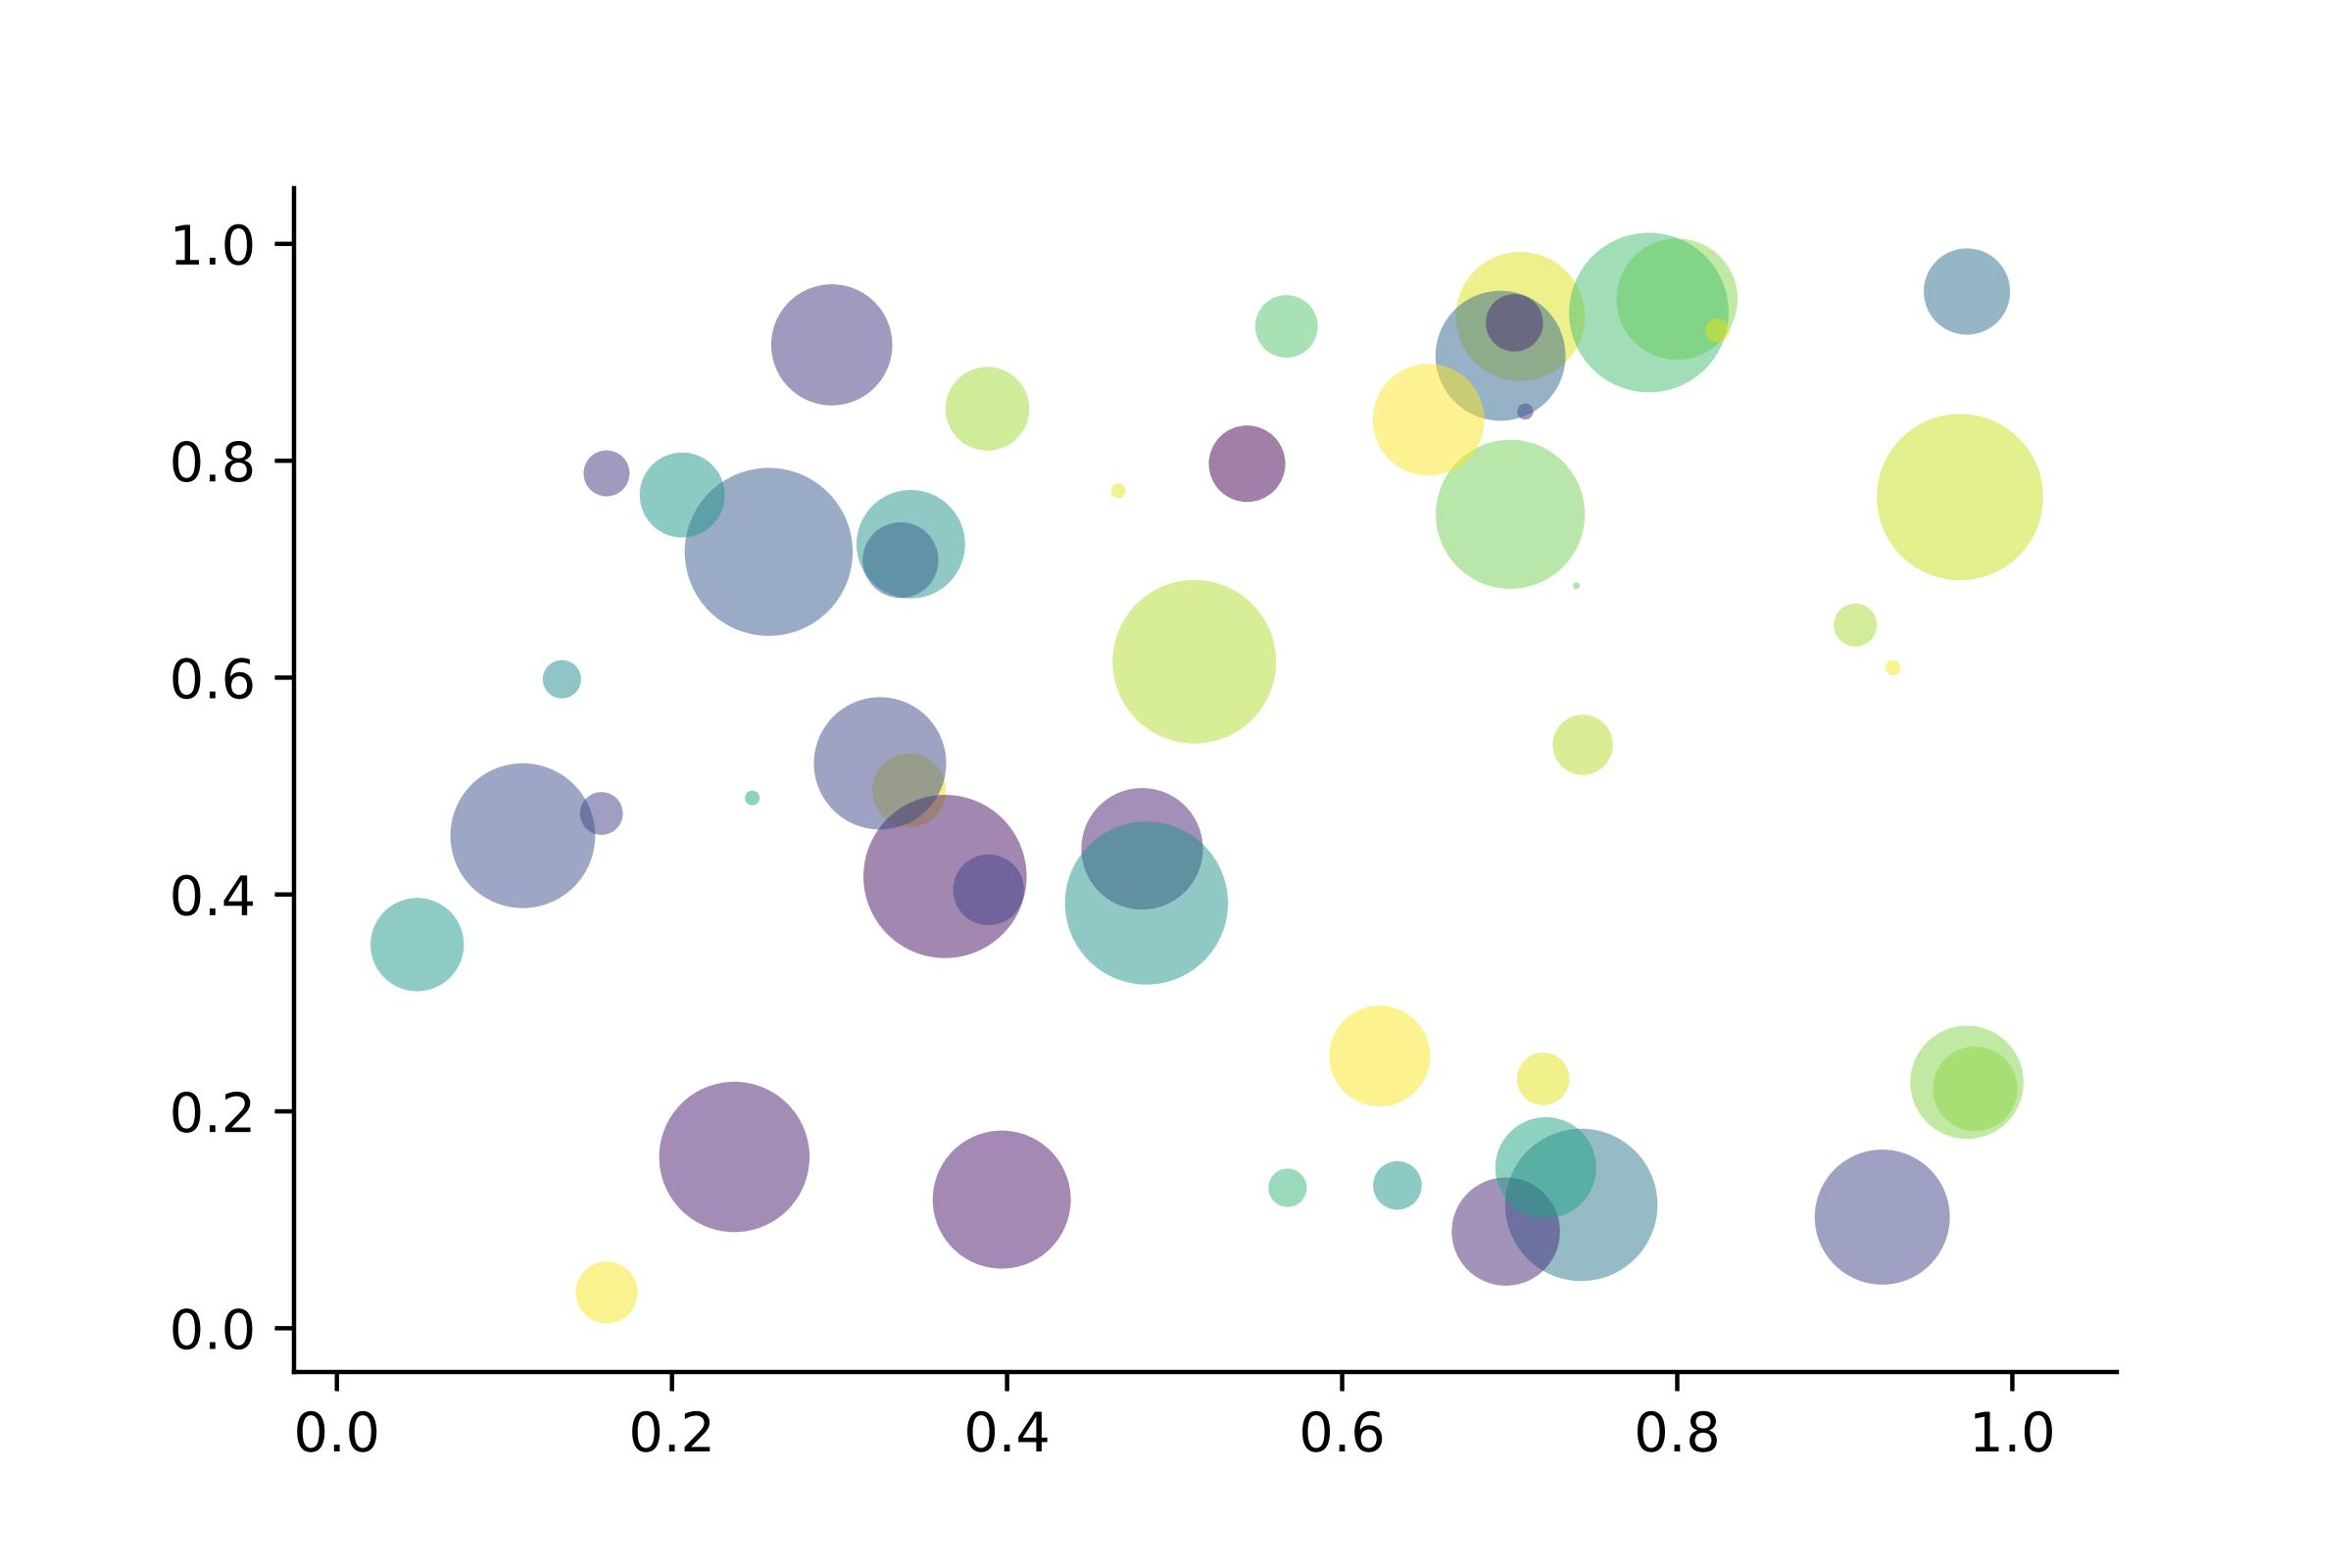
\includegraphics[width=0.6\textwidth]{scatter.jpg}
%   \caption{散点图示例 $\hat{y}=a+bx$ \label{fig:scatter}}
% \end{figure}

% 以最简单的一元线性模型来解释最小二乘法。什么是一元线性模型呢?监督学习中,如果预测的变量是离散的,我们称其为分类(如决策树,支持向量机等),如果预测的变量是连续的,我们称其为回归。回归分析中,如果只包括一个自变量和一个因变量,且二者的关系可用一条直线近似表示,这种回归分析称为一元线性回归分析。如果回归分析中包括两个或两个以上的自变量,且因变量和自变量之间是线性关系,则称为多元线性回归分析。对于二维空间线性是一条直线;对于三维空间线性是一个平面,对于多维空间线性是一个超平面。

% \begin{property}\label{property:cauchy}
% 柯西列的性质
% \begin{enumerate}
% \item $\{x_k\}$ 是柯西列,则其子列 $\{x_k^i\}$ 也是柯西列。
% \item $x_k\in \mathcal{R}^n$,$\rho(x,y)$ 是欧几里得空间,则柯西列收敛,$(\mathcal{R}^n,\rho)$ 空间是完备的。
% \end{enumerate}
% \end{property}

% \begin{conclusion}
% 回归分析(regression analysis) 是确定两种或两种以上变量间相互依赖的定量关系的一种统计分析方法。运用十分广泛,回归分析按照涉及的变量的多少,分为一元回归和多元回归分析;按照因变量的多少,可分为简单回归分析和多重回归分析;按照自变量和因变量之间的关系类型,可分为线性回归分析和非线性回归分析。
% \end{conclusion}

% \begin{problemset}
% \item 设 $A$ 为数域 $K$ 上的 $n$ 级矩阵。证明:如果 $K^n$ 中任意非零列向量都是 $A$ 的特征向量,则 $A$ 一定是数量矩阵。
% \item 证明:不为零矩阵的幂零矩阵不能对角化。
% \item 设 $A = (a_{ij})$ 是数域 $K$ 上的一个 $n$ 级上三角矩阵,证明:如果 $a_{11} = a_{22} = \cdots = a_{nn}$,并且至少有一个 $a_{kl} \not = 0 (k < l)$,则 $A$ 一定不能对角化。
% \end{problemset}

% \chapter{常见问题集}

% 我们根据用户社区反馈整理了下面一些常见的问题,用户在遇到问题时,应当首先查阅本手册和本部分的常见的问题。

% \begin{enumerate}[itemsep=1.5ex]
%   \item \question{有没有办法章节用“第一章,第一节,(一)”这种?}
%     见前文介绍,可以使用 \lstinline{scheme=chinese} 设置。
%   \item \question{大佬,我想把正文字体改为亮色,背景色改为黑灰色。}
%     页面颜色可以使用 \lstinline{\pagecolor} 命令设置,文本命令可以参考\href{https://tex.stackexchange.com/questions/278544/xcolor-what-is-the-equivalent-of-default-text-color}{这里}进行设置。
%   \item \question{\lstinline[breaklines]{Package ctex Error: CTeX fontset 'Mac' is unavailable.}}
%     在 Mac 系统下,中文编译请使用 \hologo{XeLaTeX}。
%   \item \question{\lstinline{! LaTeX Error: Unknown option 'scheme=plain' for package 'ctex'.}}
%     你用的 C\TeX{} 套装吧?这个里面的 \lstinline{ctex} 宏包已经是已经是 10 年前的了,与本模板使用的 \lstinline{ctex} 宏集有很大区别。不建议 C\TeX{} 套装了,请卸载并安装 \TeX{} Live 2022。
%   \item \question{我该使用什么版本?}
%     请务必使用\href{https://github.com/ElegantLaTeX/ElegantBook/releases}{最新正式发行版},发行版间不定期可能会有更新(修复 bug 或者改进之类),如果你在使用过程中没有遇到问题,不需要每次更新\href{https://github.com/ElegantLaTeX/ElegantBook/archive/master.zip}{最新版},但是在发行版更新之后,请尽可能使用最新版(发行版)!最新发行版可以在 GitHub 或者 \TeX{} Live 2021 内获取。
%   \item \question{我该使用什么编辑器?}
%     你可以使用 \TeX{} Live 2021 自带的编辑器 \TeX{}works 或者使用 \TeX{}studio,\TeX works 的自动补全,你可以参考我们的总结 \href{https://github.com/EthanDeng/texworks-autocomplete}{\TeX works 自动补全}。推荐使用 \TeX{} Live 2021 + \TeX{}studio。我自己用 VS Code 和 Sublime Text,相关的配置说明,请参考 \href{https://github.com/EthanDeng/vscode-latex}{\LaTeX{} 编译环境配置:Visual Studio Code 配置简介} 和 \href{https://github.com/EthanDeng/sublime-text-latex}{Sublime Text 搭建 \LaTeX{} 编写环境}。
%   \item \question{您好,我们想用您的 ElegantBook 模板写一本书。关于机器学习的教材,希望获得您的授权,谢谢您的宝贵时间。}
%     模板的使用修改都是自由的,你们声明模板来源以及模板地址(GitHub 地址)即可,其他未尽事宜按照开源协议 LPPL-1.3c。做好之后,如果方便的话,可以给我们一个链接,我把你们的教材放在 Elegant\LaTeX{} 用户作品集里。
%   \item \question{请问交叉引用是什么?}
%     本群和本模板适合有一定 \LaTeX{} 基础的用户使用,新手请先学习 \LaTeX{} 的基础,理解各种概念,否则你将寸步难行。
%   \item \question{代码高亮环境能用其他语言吗?}
%     可以的,ElegantBook 模板用的是 \lstinline{listings} 宏包,你可以在环境(\lstinline{lstlisting})之后加上语言(比如 Python 使用 \lstinline{language=Python} 选项),全局语言修改请使用 \lstinline{lsset} 命令,更多信息请参考宏包文档。
%   \item \question{群主,什么时候出 Beamer 的模板(主题),ElegantSlide 或者 ElegantBeamer?}
%     由于 Beamer 中有一个很优秀的主题 \href{https://github.com/matze/mtheme}{Metropolis}。后续确定不会再出任何主题/模板,请大家根据需要修改已有主题。
% \end{enumerate}

% \chapter{版本更新历史}

% 根据用户的反馈,我们不断修正和完善模板。由于 3.00 之前版本与现在版本差异非常大,在此不列出 3.00 之前的更新内容。


% \datechange{2022/04/09}{版本 4.3 正式发布。}

% \begin{change}
%   \item 放弃 newtx 系列宏包的设置,改用 TeX Gyre Terms,并设置其他字体;
%   \item 修改定理类环境内部字体设置,修复环境内部中文无法加粗问题;
%   \item 增加定理类环境的计数器选项 \lstinline{thmcnt},可选 \lstinline{chapter} 和 \lstinline{section};
%   \item 增加 \lstinline{bibend} 选项,可选 \lstinline{bibend=biber}(默认)和 \lstinline{bibend=bibtex}。
% \end{change}



% \datechange{2022/03/08}{版本 4.2 正式发布。}

% \begin{change}
%   \item 对于 newtx 系列宏包更新导致的字体 bug 的修复;
%   \item 修缮目录格式,为了达到这个目的,重新改写 \lstinline{\chaptername} 的重定义语句;
%   \item 增加日语 \lstinline{lang=jp} 设定。
%   \item 这个版本为一个临时性版本,在 \TeX Live 2022 发布之后,将尽快发布 4.3 版本,由于对于中文的改动比较大,可能会出现预期之外的 bug,有问题可以在 QQ 群或者 Github 反馈。
% \end{change}


% \datechange{2021/05/02}{版本 4.1 正式发布。}

% \begin{change}
%   \item \textbf{重要改动}:由原先的 \hologo{BibTeX} 改为 biblatex 编译方式(后端为 \lstinline{biber}),请注意两者之间的差异;
%   \item \textbf{重要改进}:修改对于定理写法兼容方式,提高数学公式代码的兼容性;
%   \item 页面设置改动,默认页面更宽;方便书写和阅读;
%   \item 支持目录文字以及页码跳转;
%   \item 不再维护 \hologo{pdfLaTeX} 中文支持方式,请务必使用 \hologo{XeLaTeX} 编译中文文稿。
%   \item 增加多个语言选项,法语 \lstinline{lang=fr}、荷兰语 \lstinline{lang=nl}、匈牙利语 \lstinline{lang=hu}、西班牙语 \lstinline{lang=es}、蒙古语 \lstinline{lang=mn} 等。
% \end{change}


% \datechange{2020/04/12}{版本 3.11 正式发布,\textcolor{red}{此版本为 3.x 最后版本。}}

% \begin{change}
%   \item \textbf{重要修正}:修复因为 \lstinline{gbt7714} 宏包更新导致的 \lstinline{natbib option clash} 错误;
%   \item 由于 \lstinline{pgfornament} 宏包未被 \TeX{} Live 2020 收录,因此删除 base 相关的内容;
%   \item 修复部分环境的空格问题;
%   \item 增加了意大利语言选项 \lstinline{lang=it}。
% \end{change}


% \datechange{2020/02/10}{版本 3.10 正式发布}

% \begin{change}
%   \item 增加数学字体选项 \lstinline{math},可选项为 \lstinline{newtx} 和 \lstinline{cm}。\\
%   \textbf{重要提示}:原先通过 \lstinline{newtxmath} 宏包设置的数学字体改为 \LaTeX{} 默认数学字体,如果需要保持原来的字体,需要显式声明数学字体(\lstinline{math=newtx});
%   \item 新增中文字体选项 \lstinline{chinesefont},可选项为 \lstinline{ctexfont}、\lstinline{founder} 和 \lstinline{nofont}。
%   \item 将封面作者信息设置为可选,并且增加自定义信息命令 \lstinline{\bioinfo};
%   \item 在说明文档中增加版本历史,新增 \lstinline{\datechange} 命令和 \lstinline{change} 环境;
%   \item 增加汉化章节选项 \lstinline{scheme},可选项为汉化 \lstinline{chinese};
%   \item 由于 \lstinline{\lvert} 问题已经修复,重新调整 \lstinline{ctex} 宏包和 \lstinline{amsmath} 宏包位置。
%   \item 修改页眉设置,去除了 \lstinline{\lastpage} 以避免 page anchor 问题,加入 \lstinline{\frontmatter}。
%   \item 修改参考文献选项 \lstinline{cite},可选项为数字 \lstinline{numbers}、 作者-年份 \lstinline{authoryear} 以及上标 \lstinline{super}。
%   \item 新增参考文献样式选项 \lstinline{bibstyle},并将英文模式下参考文献样式 \lstinline{apalike} 设置为默认值,中文仍然使用 \lstinline{gbt7714} 宏包设置。
% \end{change}

% \datechange{2019/08/18}{版本 3.09 正式发布}

% \begin{change}
%   \item \lstinline{\elegantpar} 存在 bug,删除 \lstinline{\elegantpar} 命令,建议用户改用 \lstinline{\marginnote} 和 \lstinline{\marginpar} 旁注命令。
%   \item 积分操作符统一更改为 \lstinline{esint} 宏包设置;
%   \item 新增目录选项 \lstinline{toc},可选项为单栏 \lstinline{onecol} 和双栏 \lstinline{twocol};
%   \item 手动增加参考文献选项 \lstinline{cite},可选项为上标形式 \lstinline{super};
%   \item 修正章节习题(\lstinline{problemset})环境。
% \end{change}

% \datechange{2019/05/28}{版本 3.08 正式发布}

% \begin{change}
%   \item 修复 \lstinline{\part} 命令。
%   \item 引入 Note 模板中的 \lstinline{pad} 选项 \lstinline{device=pad}。
%   \item 数学字体加入 \lstinline{mtpro2} 可选项 \lstinline{math=mtpro2},使用免费的 \lstinline{lite} 子集。
%   \item 将参考文献默认显示方式 \lstinline{authoyear} 改为 \lstinline{numbers}。
%   \item 引入旁注命令 \lstinline{\marginpar}(测试)。
%   \item 新增章节摘要环境 \lstinline{introduction}。
%   \item 新增章节习题环境 \lstinline{problemset}。
%   \item 将 \lstinline{\equote} 重命名为 \lstinline{\extrainfo}。
%   \item 完善说明文档,增加致谢部分。
% \end{change}

% \datechange{2019/04/15}{版本 3.07 正式发布}

% \begin{change}
%   \item 删除中英文自定义字体总设置。
%   \item 新增颜色主题,并将原绿色默认主题设置为蓝色 \lstinline{color=blue}。
%   \item 引入隐藏装饰图案选项 \lstinline{base},可选项有显示 \lstinline{show} 和隐藏 \lstinline{hide}。
%   \item 新增定理模式 \lstinline{mode},可选项有简单模式 \lstinline{simple} 和炫彩模式 \lstinline{fancy}。
%   \item 新增隐藏证明、答案等环境的选项 \lstinline{result=noanswer}。
% \end{change}

% \datechange{2019/02/25}{版本 3.06 正式发布}

% \begin{change}
%   \item 删除水印。
%   \item 新封面,新装饰图案。
%   \item 添加引言使用说明。
%   \item 修复双面 \lstinline{twoside}。
%   \item 美化列表环境。
%   \item 增加 \lstinline{\subsubsection} 的设置。
%   \item 将模板拆分成中英文语言模式。
%   \item 使用 \lstinline{lstlisting} 添加代码高亮。
%   \item 增加定理类环境使用说明。
% \end{change}

% \datechange{2019/01/22}{版本 3.05 正式发布}

% \begin{change}
%   \item 添加 \lstinline{xeCJK} 宏包中文支持方案。
%   \item 修复模板之前对 Ti\textit{k}Z 单位的改动。
%   \item 更新 logo 图。
% \end{change}

% \datechange{2019/01/15}{版本 3.04 正式发布}

% \begin{change}
%   \item 格式化模板代码。
%   \item 增加 \lstinline{\equote} 命令。
%   \item 修改 \lstinline{\date}。
% \end{change}

% \datechange{2019/01/08}{版本 3.03 正式发布}

% \begin{change}
%   \item 修复附录章节显示问题。
%   \item 小幅优化封面代码。
% \end{change}

% \datechange{2018/12/31}{版本 3.02 正式发布}

% \begin{change}
%   \item 修复名字系列命令自定义格式时出现的空格问题,比如 \lstinline{\listfigurename}。
%   \item 英文定理类名字改为中文名。
%   \item 英文结构名改为中文。
% \end{change}

% \datechange{2018/12/16}{版本 3.01 正式发布}

% \begin{change}
%   \item 调整 \lstinline{ctex} 宏包。
%   \item 说明文档增加更新内容。
% \end{change}

% \datechange{2018/12/06}{版本 3.00 正式发布}

% \begin{change}
%   \item 删除 \lstinline{mathpazo} 数学字体选项。
%   \item 添加邮箱命令 \lstinline{\mailto}。
%   \item 修改英文字体为 \lstinline{newtx} 系列,另外大型操作符号维持 cm 字体。
%   \item 中文字体改用 \lstinline{ctex} 宏包自动设置。
%   \item 删除 \lstinline{xeCJK} 字体设置,原因是不同系统字体不方便统一。
%   \item 定理换用 \lstinline{tcolobox} 宏包定义,并基本维持原有的定理样式,优化显示效果,支持跨页;定理类名字重命名,如 etheorem 改为 theorem 等等。
%   \item 删去自定义的缩进命令 \lstinline{\Eindent}。
%   \item 添加参考文献宏包 \lstinline{natbib}。
%   \item 颜色名字重命名。
% \end{change}

% \nocite{*}
% \printbibliography[heading=bibintoc, title=\ebibname]
% \appendix

% \chapter{基本数学工具}


% 本附录包括了计量经济学中用到的一些基本数学,我们扼要论述了求和算子的各种性质,研究了线性和某些非线性方程的性质,并复习了比例和百分数。我们还介绍了一些在应用计量经济学中常见的特殊函数,包括二次函数和自然对数,前 4 节只要求基本的代数技巧,第 5 节则对微分学进行了简要回顾;虽然要理解本书的大部分内容,微积分并非必需,但在一些章末附录和第 3 篇某些高深专题中,我们还是用到了微积分。

% \section{求和算子与描述统计量}

% \textbf{求和算子} 是用以表达多个数求和运算的一个缩略符号,它在统计学和计量经济学分析中扮演着重要作用。如果 $\{x_i: i=1, 2, \ldots, n\}$ 表示 $n$ 个数的一个序列,那么我们就把这 $n$ 个数的和写为:

% \begin{equation}
% \sum_{i=1}^n x_i \equiv x_1 + x_2 +\cdots + x_n
% \end{equation}



\end{document}
